\documentclass[12pt]{article}
\usepackage[utf8]{inputenc}
\usepackage{polski}
\usepackage{listing}
\usepackage{listings}
\usepackage{amsmath}
\usepackage{multicol}
\usepackage{graphicx}
\usepackage[shortlabels]{enumitem}
\graphicspath{ {./images/} }
\title{
	Obliczenia naukowe \\
	Sprawozdanie 4
}
\addtolength{\oddsidemargin}{-.8in}
\addtolength{\evensidemargin}{-.8in}
\addtolength{\textwidth}{1.75in}
\addtolength{\topmargin}{-.7in}
\addtolength{\textheight}{1.75in}

\date{7 grudnia 2019}
\author{Józef Piechaczek}

\begin{document}

\pagenumbering{gobble}
\maketitle
\newpage
\pagenumbering{arabic}

\setlength{\abovedisplayskip}{5pt}
\setlength{\belowdisplayskip}{5pt}

\section{Zadanie 1}
Celem zadania 1 jest napisanie funkcji obliczającej ilorazy różnicowe.\\
\textbf{Definicja funkcji:}

\begin{verbatim}
function ilorazyRoznicowe (x::Vector{Float64}, f::Vector{Float64})
\end{verbatim}
\textbf{Dane:}
\begin{itemize}[leftmargin=4.0cm,labelsep=0.4cm]
\item[$x$] wektor długości $n + 1$ zawierający węzły $x_0, ..., x_n$ \texttt{x[1]}=$x_0$,...,\texttt{x[n+1]}=$x_n$
\item[$f$] wektor długości $n+1$ zawierający wartości interpolowanej funkcji w węzłach $f(x_0),...,f(x_n)$
\end{itemize}
\textbf{Wyniki:} 
\begin{itemize}[leftmargin=4.0cm,labelsep=0.4cm]
\item[$fx$] wektor długości $n+1$ zawierający obliczone ilorazy różnicowe \\
\texttt{fx[1]}=$f[x_0]$\\
\texttt{fx[2]}=$f[x_0, x_1]$,...,\texttt{fx[n+1]}=$f[x_0,...,x_n]$
\end{itemize}

\noindent Funkcję należy zaprojektować bez użycia tablicy dwuwymiarowej.
\\
\\
\noindent \textbf{Opis algorytmu:}\\
W celu obliczenia ilorazów korzystamy z następujących zależności:
\begin{enumerate}[I.]
\item $f[x_i]=f(x_i)$ dla $0 \leq i \leq n$
\item $f[x_i, \ldots , x_{i+j+1}] = \frac{f[x_{i+1}, \ldots , x_{i+j+1}] - f[x_i, \ldots , x_{i+j}]}{x_{i+j+1}-x_i}$
\end{enumerate}

\noindent Ilorazy różnicowe możemy łatwo policzyć korzystając z tablicy trójkątnej tworzonej w następujący sposób:
\begin{center}
\minipage{0.69\textwidth}
  \begin{align*}
&  x_0    & &f[x_0]     & &f[x_0, x_1] 			& &f[x_0, x_1, x_2] & &\hdots & &f[x_0, \ldots, x_n]\\
&  x_1    & &f[x_1]     & &f[x_1, x_2] 			& &f[x_1, x_2, x_3]\\
&  x_2    & &f[x_2]     & &f[x_2, x_3] 			& &f[x_2, x_3, x_4]\\
& \vdots  & &\vdots     & &\vdots				& &\vdots\\
& x_{n-2} & &f[x_{n-2}] & &f[x_{n-2}, x_{n-1}]	& &f[x_{n-2}, x_{n-1}, x_n]\\
& x_{n-1} & &f[x_{n-1}] & &f[x_{n-1}, x_n] 		& &\\
& x_n     & &f[x_n]     & & \\
\end{align*}
\endminipage\hfill
\end{center}

\noindent Do przechowywania wartości ilorazów wystarczy zwykła tabela, której początkowymi wartościami, będą wartości funkcji w interpolowanych węzłach. W i-tej iteracji zewnętrznej pętli algorytmu będziemy modyfikować wartości w tablicy od $n$ do $i$.
\\
\\
\noindent \textbf{Algorytm:}
\begin{verbatim}
l <- length(x)
fx <- f
for j=2 to l do
  for i=l downto j do
    fx[i] <- (fx[i] - fx[i - 1])/(x[i] - x[i - j + 1])
return fx
\end{verbatim}

\section{Zadanie 2}
Napisać funkcję obliczającą wartość wielomianu interpolacyjnego stopnia $n$ w postaci Newtona $N_n(x)$ w punkcie $x=t$ za pomocą uogólnionego algorytmu Hornera, w czasie $O(n)$.\\
\textbf{Definicja funkcji:}

\begin{verbatim}
function warNewton (x::Vector{Float64}, fx::Vector{Float64}, t::Float64)
\end{verbatim}
\textbf{Dane:}
\begin{itemize}[leftmargin=4.0cm,labelsep=0.4cm]
\item[$x$] wektor długości $n + 1$ zawierający węzły $x_0, ..., x_n$ \texttt{x[1]}=$x_0$,...,\texttt{x[n+1]}=$x_n$
\item[$fx$] wektor długości $n+1$ zawierający ilorazy różnicowe \\
\texttt{fx[1]}=$f[x_0]$\\
\texttt{fx[2]}=$f[x_0, x_1]$,...,\texttt{fx[n+1]}=$f[x_0,...,x_n]$
\end{itemize}
\textbf{Wyniki:} 
\begin{itemize}[leftmargin=4.0cm,labelsep=0.4cm]
\item[$nt$] wartość wielomianu w punkcie $t$ \\
\end{itemize}

\noindent \textbf{Opis algorytmu:}\\
W celu obliczenia wartości wielomianu interpolacyjnego w punkcie użyjemy uogólnionego algorytmu Hornera.
\begin{align*}
	w_n(x) &:= f[x_0, x_1, \ldots, x_n] \\
	w_k(x) &:= f[x_0, \ldots, x_k] + (x - x_k)w_{k+1}(x) \qquad (k = n-1, \ldots, 0) \\
	N_n(x) &:= w_0(x)
\end{align*}

\noindent Podane wzory wynikają z następującej postaci Newtona wielomianu interpolacyjnego 
\begin{align*}
N_n(x) &= \sum_{j=0}^n c_jq_j(x) \\
c_j &= f[x_0, \ldots, x_j] \\
q_j &= \prod_{i=0}^{j-1} (x-x_i)
\end{align*}

\noindent Algorytm działa w czasie $O(n)$.

\noindent \textbf{Algorytm:}
\begin{verbatim}
l <- length(x)
nt = fx[l]
for i=l-1 downto 1
  nt = fx[i] + (t - x[i]) * nt
return nt
\end{verbatim}

\clearpage

\section{Zadanie 3}
Znając współczynniki wielomianu interpolacyjnego w postaci Newtona $c_0=f[x_0], c_1=f[x_0, x_1], c_2=f[x_0, x_1, x_2], \ldots ,c_n=f[x_0, \ldots , x_n]$(ilorazy różnicowe) oraz węzły $x_0, x_1, \ldots , x_n$ napisać funkcję obliczającą, w czasie $O(n^2)$, współczynniki jego postaci naturalnej $a_0, \ldots , a_n$ tzn. $a_nx_n+a_{n-1}x^{n-1}+ \ldots +a_1x+a_0$.\\
\textbf{Definicja funkcji:}
\begin{verbatim}
function naturalna (x::Vector{Float64}, fx::Vector{Float64})
\end{verbatim}

\noindent \textbf{Dane:}
\begin{itemize}[leftmargin=4.0cm,labelsep=0.4cm]
\item[$x$] wektor długości $n + 1$ zawierający węzły $x_0, ..., x_n$ \texttt{x[1]}=$x_0$,...,\texttt{x[n+1]}=$x_n$
\item[$fx$] wektor długości $n+1$ zawierający ilorazy różnicowe \\
\texttt{fx[1]}=$f[x_0]$\\
\texttt{fx[2]}=$f[x_0, x_1]$,...,\texttt{fx[n+1]}=$f[x_0,...,x_n]$
\end{itemize}
\textbf{Wyniki:} 
\begin{itemize}[leftmargin=4.0cm,labelsep=0.4cm]
\item[$a$] wektor długości $n + 1$ zawierający obliczone współczynniki postaci naturalnej \\
\texttt{a[1]} = $a_0$\\
\texttt{a[2]} = $a_1$, \ldots, \texttt{a[n]}=$a_{n-1}$, \texttt{a[n+1]}=$a_n$
\end{itemize}

\noindent \textbf{Opis algorytmu:}\\
Algorytm korzysta z uogólnionego algorytmu Hornera z poprzedniego zadania. Jako $a_n$ przyjmujemy wartość $f[x_0, \ldots, x_n]$, co da się łatwo wykazać. Następnie w każdej iteracji zewnętrznej pętli obliczamy częściową wartość dla wielomianu, podobnie jak w zadaniu 2, a w wewnętrznej pętli aktualizujemy wartości współczynników tak, aby częściowy wielomian $w_k$ był w postaci naturalnej. Algorytm działa w czasie $O(n^2)$.

\noindent \textbf{Algorytm:}
\begin{verbatim}
l <- length(x)
a[l] <- fx[l]
for i = (l-1) downto 1
  a[i] = fx[i] - a[i+1] * x[i]
  for j = (i+1) to (l-1)
    a[j] = a[j] - a[j+1] * x[i]
return a
\end{verbatim}

\section{Zadanie 4}
Napisać funkcję, która zinterpoluje zadaną funkcję $f(x)$ w przedziale $[a, b]$ za pomocą wielomianu interpolacyjnego stopnia $n$ w postaci Newtona. Następnie narysuje wielomian interpolacyjny i interpolowaną funkcję. W interpolacji użyć węzłów równoodległych, tj. $x_k=a+kh, h=\frac{b-a}{n}, k= 0,1, \ldots , n$. Nie wyznaczać wielomianu interpolacyjnego w jawnej postaci. Należy skorzystać z funkcji \texttt{ilorazyRoznicowe} i \texttt{warNewton}.


\noindent \textbf{Definicja funkcji:}

\begin{verbatim}
function rysujNnfx(f,a::Float64,b::Float64,n::Int)
\end{verbatim}

\noindent \textbf{Dane:}
\begin{itemize}[leftmargin=4.0cm,labelsep=0.4cm]
\item[$f$] funkcja $f(x)$ zadana jako anonimowa funkcja
\item[$a, b$]  przedział interpolacji
\item[$n$] stopień wielomianu interpolacyjnego
\end{itemize}
\textbf{Wyniki:} 
\begin{itemize}[leftmargin=4.0cm,labelsep=0.4cm]
\item[] wykres funkcji interpolowanej i wielomianu interpolacyjnego na przedziale $[a,b]$
\end{itemize}


\noindent \textbf{Opis rozwiązania:}\\
Algorytm dzieli przedział $[a,b]$ na $n+1$ równo odległych punktów i oblicza wartość funkcji w tych punktach. Następnie korzysta z funkcji \texttt{ilorazyRoznicowe} w celu obliczenia ilorazów różnicowych. Następnie program dzieli zadany przedział na równo odległe punkty z większym zagęszczeniem (w celu większej dokładności wykresu) i oblicza wartości funkcji interpolowanej i wielomianu interpolującego (za pomocą \texttt{warNewton}) w tych punktach. Wykresy są tworzone za pomocą biblioteki \textbf{Plots} i zapisywane do pliku.

\section{Zadanie 5}
Przetestować funkcję \texttt{rysujNnfx(f,a,b,n)} na następujących przykładach:
\begin{enumerate}[(a)]
	\item $e^x, [0,1], n=5,10,15$
	\item $x^2sin x, [-1, 1], n=5,10,15$
\end{enumerate}


\noindent \textbf{Rozwiązania:}
\clearpage

\begin{figure}[!htb]
\minipage{0.49\textwidth}
  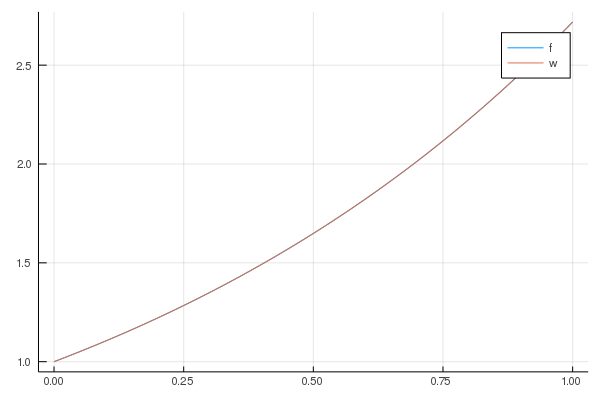
\includegraphics[width=\linewidth]{myplot_1_5.png}
  \caption{$e^x, n=5$}
\endminipage\hfill
\minipage{0.49\textwidth}
  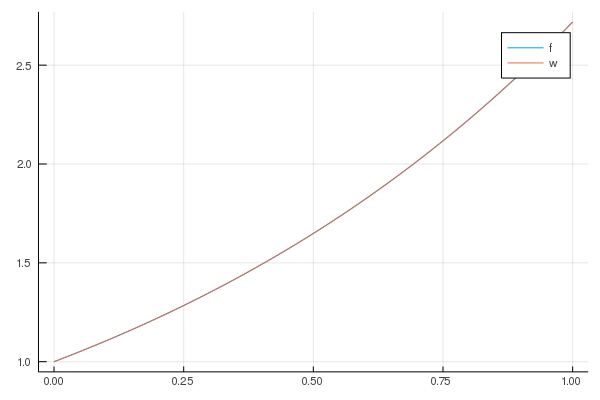
\includegraphics[width=\linewidth]{myplot_1_10.png}
  \caption{$e^x, n=10$}
\endminipage
\end{figure}
\begin{figure}[!htb]
\minipage{0.49\textwidth}
  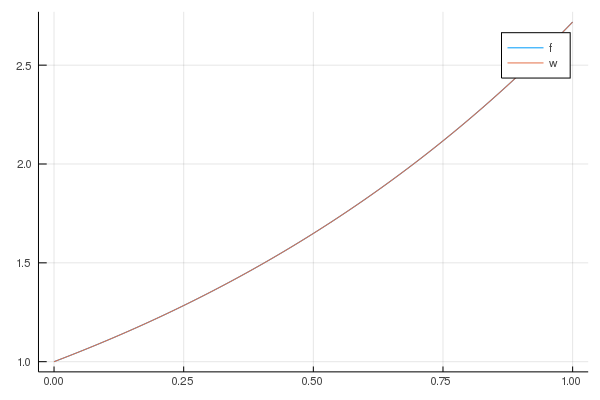
\includegraphics[width=\linewidth]{myplot_1_15.png}
  \caption{$e^x, n=15$}
\endminipage\hfill
\minipage{0.49\textwidth}
  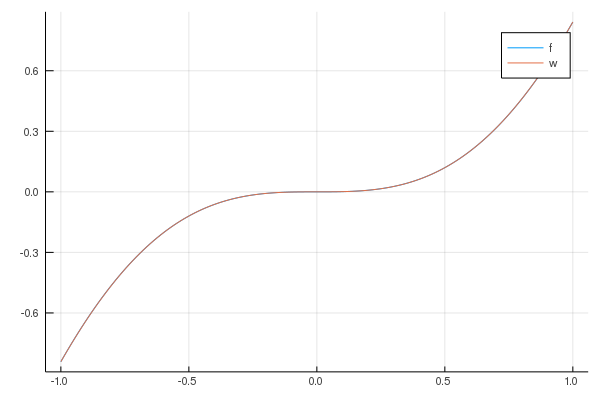
\includegraphics[width=\linewidth]{myplot_2_5.png}
  \caption{$x^2sin x, n=5$}
\endminipage
\end{figure}
\begin{figure}[!htb]
\minipage{0.49\textwidth}
  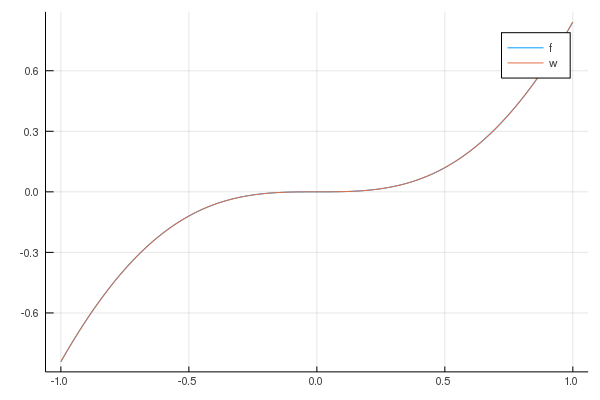
\includegraphics[width=\linewidth]{myplot_2_10.png}
  \caption{$x^2sin x, n=10$}
\endminipage\hfill
\minipage{0.49\textwidth}
  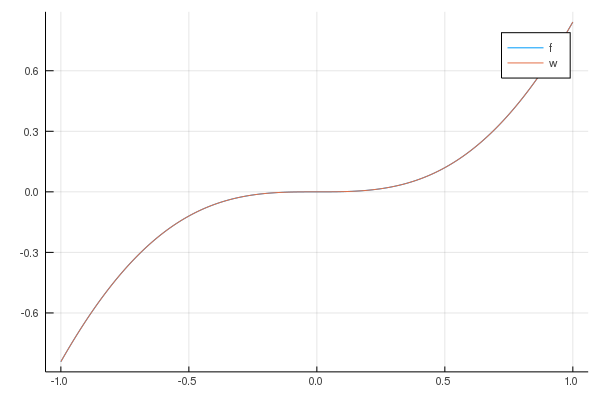
\includegraphics[width=\linewidth]{myplot_2_15.png}
  \caption{$x^2sin x, n=15$}
\endminipage
\end{figure}



\clearpage
\noindent \textbf{Wnioski:}\\
Patrząc na wykresy funkcji można zauważyć że zadane wielomiany bardzo dobrze interpolują podane funkcje. Nawet dla wielomianu stopnia $n=5$ nie da się zobaczyć rozbieżności na wykresach.

\section{Zadanie 6}
Przetestować funkcję \texttt{rysujNnfx(f,a,b,n)} na następujących przykładach:
\begin{enumerate}[(a)]
	\item $|x|, [-1,1], n=5,10,15$
	\item $\frac{1}{1+x^2}, [-5, 5], n=5,10,15$
\end{enumerate}


\noindent \textbf{Rozwiązania:}
\begin{figure}[!htb]
\minipage{0.49\textwidth}
  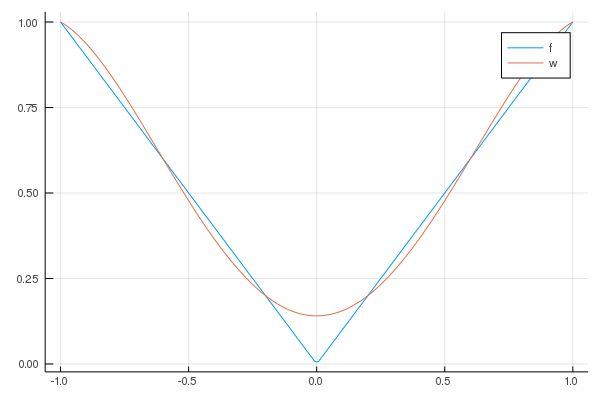
\includegraphics[width=\linewidth]{myplot_3_5.png}
  \caption{$|x|, n=5$}
\endminipage\hfill
\minipage{0.49\textwidth}
  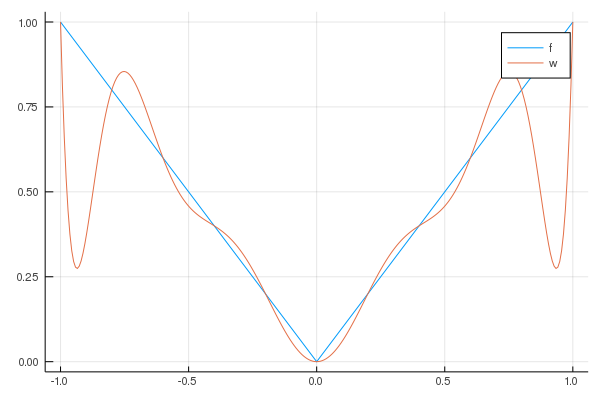
\includegraphics[width=\linewidth]{myplot_3_10.png}
  \caption{$|x|, n=10$}
\endminipage
\end{figure}
\begin{figure}[!htb]
\minipage{0.49\textwidth}
  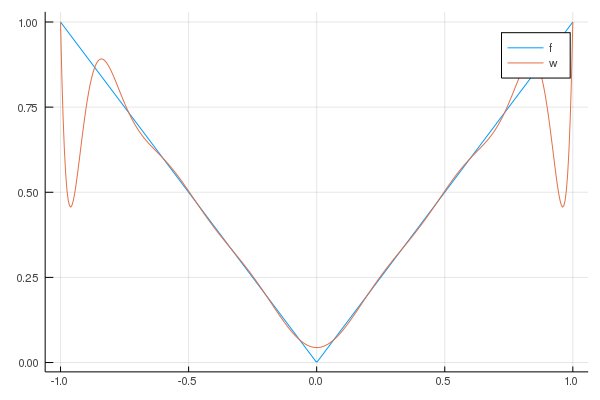
\includegraphics[width=\linewidth]{myplot_3_15.png}
  \caption{$|x|, n=15$}
\endminipage\hfill
\minipage{0.49\textwidth}
  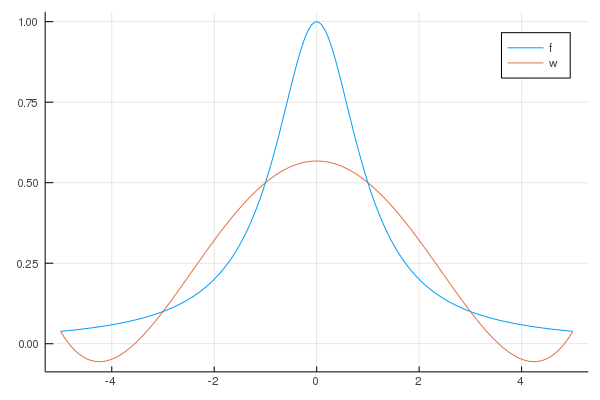
\includegraphics[width=\linewidth]{myplot_4_5.png}
  \caption{$\frac{1}{1+x^2}, n=5$}
\endminipage
\end{figure}
\clearpage
\begin{figure}[!htb]
\minipage{0.49\textwidth}
  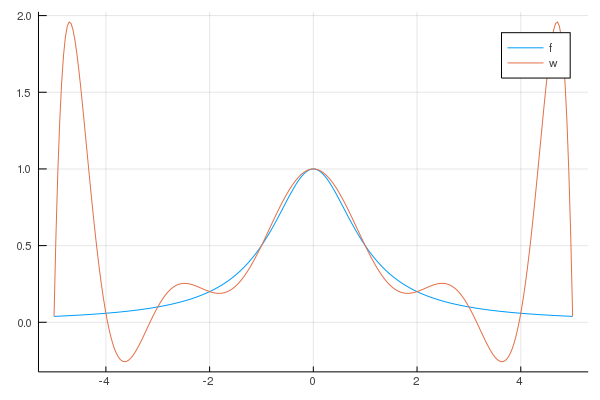
\includegraphics[width=\linewidth]{myplot_4_10.png}
  \caption{$\frac{1}{1+x^2}, n=10$}
\endminipage\hfill
\minipage{0.49\textwidth}
  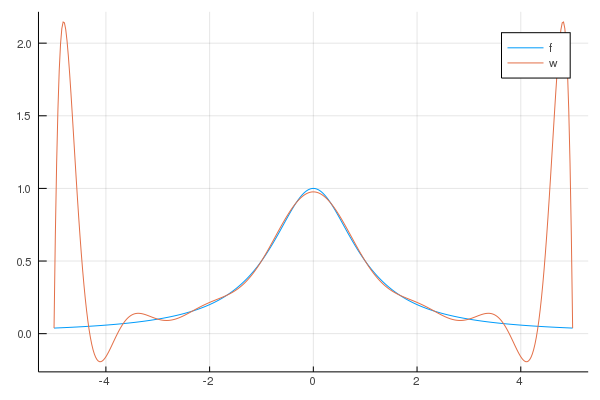
\includegraphics[width=\linewidth]{myplot_4_15.png}
  \caption{$\frac{1}{1+x^2}, n=15$}
\endminipage
\end{figure}

\noindent \textbf{Wnioski:}\\
W przypadku wielomianów interpolujących w zadaniu 6 możemy zauważyć, że wraz ze wzrostem stopnia wielomianu jakość interpolacji ulega pogorszeniu. Jest to szczególnie widoczne na końcach przedziałów. W wypadku pierwszym wynika to z faktu, że funkcja znacząco odbiega od funkcji gładkiej. W drugim przykładzie
 możemy zaobserwować efekt Rungego, który jest zjawiskiem typowym dla interpolacji za pomocą wielomianów wysokich stopni przy stałych odległościach węzłów. Aby uniknąć tego efektu, możemy stosować interpolację z węzłami upakowanymi gęściej na krańcach przedziału interpolacji.






\end{document}